\chapter{Results}
\label{chp4}

\paragraph{ }In this chapter all results obtained from analysing the data and running the anomaly detection algorithms will be presented. 

\section{Beam Displacement Over Time}

\begin{figure}[!b]
	\begin{minipage}[b]{0.475\linewidth}
		\centering
		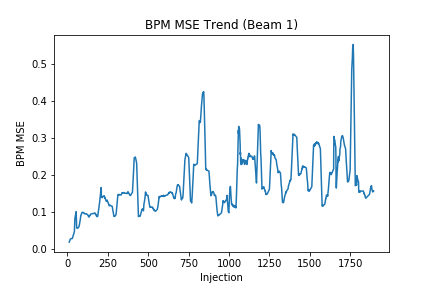
\includegraphics[width=\textwidth]{BPM_MSE_Trend_B1}
		\caption[BPM MSE Trend B1]{Trend Component of the BPM MSE for Beam 1}
		\label{fig::BPM_MSE_Trend_B1}
	\end{minipage}	
	\hspace{0.25cm}
	\begin{minipage}[b]{0.475\linewidth}
		\centering
		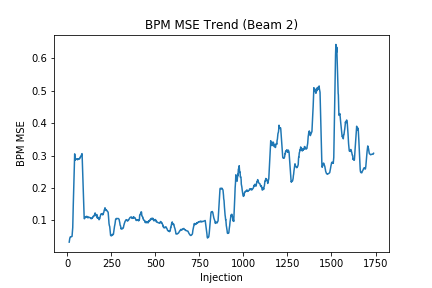
\includegraphics[width=\textwidth]{BPM_MSE_Trend_B2}
		\caption[BPM MSE Trend B2]{Trend Component of the BPM MSE for Beam 2}
		\label{fig::BPM_MSE_Trend_B2}
	\end{minipage}	
\end{figure}

\paragraph{ }When performing the initial analysis on the provided \acs{BPM} data, the \acs{MSE} of the Beam's Position with respect to its initial position in the first injection was calculated (refer to Section \ref{sec::Data_Cleaning_and_Analysis}). A rolling average of the time series points was taken to visualise the trend component. The window size was taken to be 12 since 12 injections are needed to fill the \acs{LHC}. Figures \ref{fig::BPM_MSE_Trend_B1} and \ref{fig::BPM_MSE_Trend_B2} show the trend component for Beam 1 and Beam 2 respectively. Although there's some noise in the data, it is clear from both plots that the Beam's position drifts with time.

\paragraph{ }This result confirms the suspicion that the beam position in the transfer line changes over time, which could have an impact on the injection quality. The cause of this phenomenon is due to ground motion as the slightest movement in one of the \acs{LHC}'s quadrupole magnets can throw off the beam's precision. Thus regular servicing and maintenance of the \acs{LHC} is important to reduce the number of anomalous injections.

\paragraph{ }First order differencing was then done on the data to remove the trend component. The resulting plots can be seen in Figures \ref{fig::BPM_MSE_Diff_B1} and \ref{fig::BPM_MSE_Diff_B2}. From these plots we can conclude that the spikes in the \acs{MSE} values are not cyclic but merely random.

\begin{figure}[!t]
	\begin{minipage}[b]{0.475\linewidth}
		\centering
		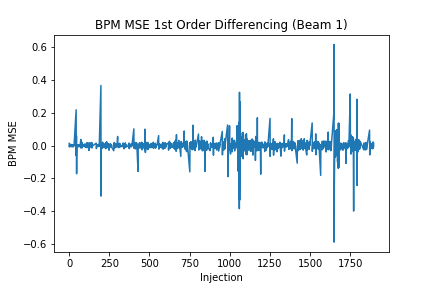
\includegraphics[width=\textwidth]{BPM_MSE_Diff_B1}
		\caption[BPM MSE Differencing B1]{1st Order Differencing for the BPM MSE for Beam 1}
		\label{fig::BPM_MSE_Diff_B1}
	\end{minipage}	
	\hspace{0.25cm}
	\begin{minipage}[b]{0.475\linewidth}
		\centering
		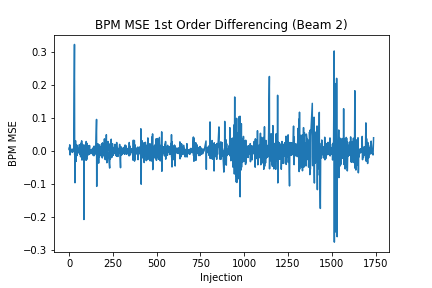
\includegraphics[width=\textwidth]{BPM_MSE_Diff_B2}
		\caption[BPM MSE Differencing B2]{1st Order Differencing for the BPM MSE for Beam 2}
		\label{fig::BPM_MSE_Diff_B2}
	\end{minipage}	
\end{figure}

\section{Performance of the Anomaly Detection Algorithms}

\paragraph{ }After running all the algorithms as described in Section \ref{sec::AnomalyDetection}, a total of 131 unique anomalous injections were detected for Beam 1. After manual inspection of each injection by Prof. Valentino, 90 (68.70\%) of these points were found to be actual anomalies. Furthermore, a total of 232 unique anomalous injections were detected for Beam 2, where 134 (57.76\%) of these were found to be actual anomalies. Since we do not know the actual number of anomalous injections that happened over the analysed time period, it must be assumed that these are all the anomalous injections and compare the performance of the different algorithms based off of these points.

\subsection{3D \acs{LOF}}

\paragraph{ }Of the  60 injections detected as anomalies by the 3D \acs{LOF} algorithm for Beam 1, 39 of these were found to be actual anomalies (65\%). These detected points can be seen in Figure \ref{fig::3D_results1} where the green points represent the correctly classified injections and the red points represent the false-positives generated. The 2D plots in \ref{fig::3D_results2} and \ref{fig::3D_results3} highlight the nature of these anomalies more clearly. 

\paragraph{ }Of the 98 injections detected as anomalies by the 3D \acs{LOF} algorithm for Beam 2, 45 of these were found to be actual anomalies (45.91\%). These detected points can be seen in Figure \ref{fig::3D_results1_B2}.

\paragraph{ }As can be clearly seen from these plots, performing \acs{LOF} on this 3 dimensional dataset is not sufficient to explain the causes for anomalies as many points that are clearly outliers and being detected as anomalies are not anomalous injections after all. The algorithm still performed reasonably well however and adding more dimensions might improve its performance.

\begin{figure}[h]
	\centering
	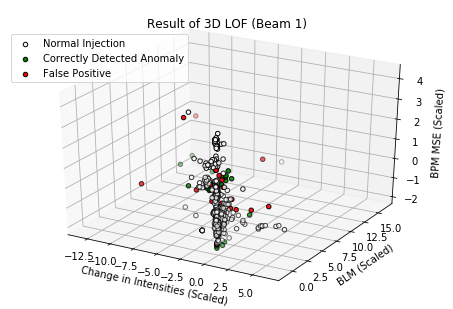
\includegraphics[width=0.8\textwidth]{3D_LOF_Results}
	\caption[3D LoF Results Beam 1]{3D Plot Highlighting Anomalies Detected by the 3D LOF Algorithm for Beam 1}
	\label{fig::3D_results1}
\end{figure}  


\begin{figure}[H]
	\centering
	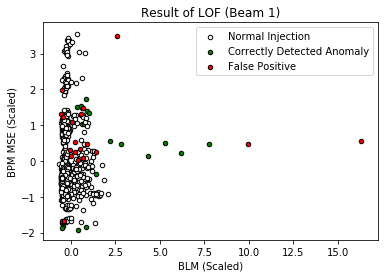
\includegraphics[width=0.8\textwidth]{3D_LOF_BLMBPM}
	\caption[3D LoF Results 2]{Anomalies Detected by the 3D LOF Algorithm}
	\label{fig::3D_results2}
\end{figure}  

\begin{figure}[H]
	\centering
	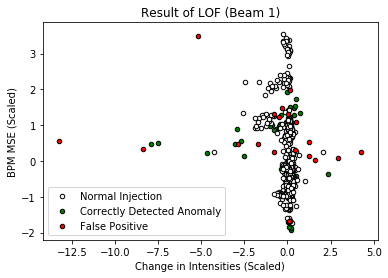
\includegraphics[width=0.8\textwidth]{3D_LOF_ResultsBPMIntensity}
	\caption[3D LoF Results 2]{Anomalies Detected by the 3D LOF Algorithm}
	\label{fig::3D_results3}
\end{figure} 

\begin{figure}[H]
	\centering
	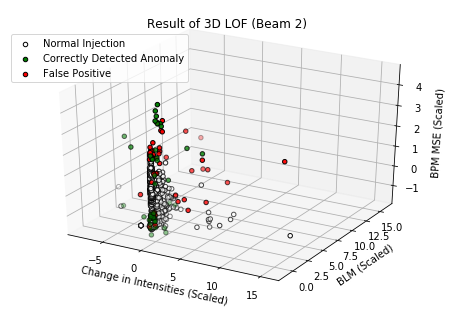
\includegraphics[width=0.8\textwidth]{Beam2_3D_LOF_Results}
	\caption[3D LoF Results Beam 2]{3D Plot Highlighting Anomalies Detected by the 3D LOF Algorithm for Beam 2}
	\label{fig::3D_results1_B2}
\end{figure}  

\subsection{3D \acs{DBSCAN}}
